\documentclass[
  convert={outext=.svg,command=\unexpanded{pdf2svg \infile\space\outfile}}
]{standalone}

\usepackage{tikz}
\usetikzlibrary{bayesnet}

\begin{document}

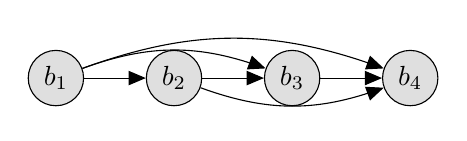
\begin{tikzpicture}[]
  \node[obs] (b1) at (0,0) {$b_1$};
  \node[obs] (b2) at (1.5,0) {$b_2$};
  \node[obs] (b3) at (3,0) {$b_3$};
  \node[obs] (b4) at (4.5,0) {$b_4$};
  \edge {b1} {b2};
  \draw[bend left=20,->] (b1) to (b3);
  \draw[bend left=20,->] (b1) to (b4);
  \edge {b2} {b3};
  \draw[bend right=20,->] (b2) to (b4);
  \edge {b3} {b4};
\end{tikzpicture}

\end{document}
%%% Local Variables:
%%% TeX-command-extra-options: "-shell-escape"
%%% End: